\makeatletter
\def\input@path{{../}}
\makeatother
\documentclass[../main.tex]{subfiles}

\newcommand{\loss}{\mathcal{L}{[f_{w} (x_{\mu}), y_{\mu}]}}

\begin{document}
\section{Introduction}
Broadly speaking, the subject of \emph{machine learning} (ML), refers to the automated detection of meaningful patterns
in data~\cite{shalev2014understanding}, and encompasses two major classes of problems: \emph{estimation} and
\emph{prediction}. 
%
% In particular, ML is concerned with two major classes of problems, \emph{estimation} and \emph{prediction}.
%
To better understand the difference between the two, we begin with an example.
%
Suppose we observe some observable quantity $x$ (e.g.\ measurements of the acceleration of an object in a
gravitational field) of the system under consideration that is related to some parameters $w$ (e.g.\ the
gravitational constant) of a model $p (x | w)$ that describes the probability of observing $x$ given
$w$.
%
We can perform an experiment to obtain a datset $x$, and use this data to ``fit'' our model. This procedure of
fitting the model typically corresponds to finding the $\hat w$ that maximizes the probability of observing
$x$, i.e.\ $\hat{w} \equiv \mathrm{argmax}_{w} \{p (x|w)\}$.
%
In this context, \emph{estimation} problems are those concerned with the accuracy of $\hat{w}$, whereas
\emph{prediction} problems are concerned with the ability of the model to predict new observations, i.e.\ the accuracy
of $p (x|\hat{w})$.

For our purposes, we mainly restrict our attention to \emph{prediction}-type problems, which includes the types of
problems most frequently associated with machine learning (i.e.\ regression, classification, etc.).
% In what follows, we will restrict our attention to \emph{prediction}-type problems, but for those interested
% More specifically, it is useful to define three generic classes of learning problems:
There are three generic approaches commonly used to tackle these types of problems, namely: 
%
\begin{enumerate}
  \item Supervised learning
  \item Unsupervised learning
  \item Reinforcement learning
\end{enumerate}
%
While it is true that most machine learning problems fit nicely into one of these three categories, this is not always
the case.
%
Some of the most successful approaches to historically difficult problems have employed ideas from combinations of the
three in new and unexpected ways (e.g.\ \emph{variational auto-encoders} (VAEs)~\cite{kingma2013auto}, and
\emph{generative adversarial networks} (GANs)~\cite{goodfellow2014generative}).
\section{Supervised Learning and Gradient Descent}%
\label{sec:supervised_learning_gradient_descent}
Supervised learning is the task of inferring a function from labeled training data.
%
Our training data consists of (input, output) pairs: $\{(x^{(i)}, y^{(i)})\}, i = 1, \ldots, n$, with $x^{(i)} \in
\mathbb{R}^{p}$ being the inputs (or features) and $y^{(i)} \in \mathbb{R}^{d}$, being the outputs (or target) (often
$d = 1$) that we wish to predict.\footnote{Here superscript $(i)$ indexes samples in the training set.}
%
For concreteness, suppose we have a collection of $n$ two-dimensional greyscale images, $x^{(1)}, x^{(2)}, \ldots,
x^{(n)}$, each of which contains $p$ pixels flattened into a vector, and their associated labels $y^{(1)}, y^{(2)},
\ldots, y^{(n)}$ matching the type of animal present in the image (e.g.\ dog, cat, frog, etc).
%
Our goal then is to find a function $f$ that is able to accurately approximate the output $y^{(i)}$ for a given input
$x^{(i)}$.
%
If our output is discrete, as in the present case, the problem is said to be a \emph{classification} problem, whereas
continuous outputs are referred to as \emph{regression} problems.
%
In order to measure how well our function performs, we often split the available data into two disjoint sets called the
training set and test set respectively.
%
The idea is to train our function (using a suitably chosen procedure) on the training data and then use the (previously
unseen) data from the test set to evaluate the performance.
%
The ability to accurately predict the desired output for a new, unused input is known as \emph{generalizability} and is
an important metric for measuring the quality of a given model.

In order to find this desired function $f_w$, we must introduce a way to measure the similarity between the expected
($y^{(i)}$) and predicted output $f_{w}(x^{(i)})$.
%
One way to to this is to introduce a \emph{loss} (or \emph{cost}) function, $\mathcal{L} =
\mathcal{L}[f_{w}(x^{(i)}), y^{(i)}] \equiv \mathcal{L}(w)$, with the idea being that the loss is small when $f_{w}(x^{(i)})
\simeq y^{(i)}$.
%
In doing so, we are able to improve the quality of our desired function $f_w$ by adjusting the values of $w$ in such a
way that the loss function is minimized.
%
One of the most popular techniques for carrying out this optimization is an algorithm known as \textbf{gradient
descent}.
%
Explicitly, given some initial (often random) values of the parameters $w$, gradient descent repeatedly updates their
values by ``stepping'' in the direction of steepest decrease of $\mathcal{L}$:
%
\begin{equation}
  w_{j} := w_{j} - \alpha \frac{\partial}{\partial w_{j}} \mathcal{L}(w), %\quad (\forall\,\, j = 0, \ldots, n).
\end{equation}
%
simultaneously for all values of $j = 0, \ldots, n$.

Here, $\alpha$ is a \emph{hyperparameter} called the \textbf{learning rate}, and it is responsible for determining the
``step size'' the algorithm takes with each update.
%
Its important to note that the value of the learning rate must be chosen appropriately since large steps can
potentially cause stability issues (resulting from `over-shooting' the minima), whereas taking steps which are too
small can dramatically increase the amount of updates necessary to obtain the minimum.
%
\subsection{Example: Linear Regression}%
\label{subsec:linear_regression}
To make all of these ideas explicit we consider the example of \emph{linear regression}. 
We begin by assuming that, to good approximation, $y$ can be expressed as a linear function of $x$:
%
\begin{equation}
  f_{w}(x) = \sum_{i=0}^{n} w_{i} x_{i} = w^{T} x
\end{equation}
%
where we've defined $x_{0} \equiv 1$ as the intercept (or \emph{bias}) term.

Next, we must choose a loss function $\mathcal{L}$.
%
For this example, we can choose the least-squares cost function defined to be
%
\begin{equation}
  \mathcal{L}(w) = \frac{1}{2}\sum_{i = 1}^{m} {\left(f_{w} (x_{i}) - y_{i} \right)}^{2}.
\end{equation}
%
In order to implement gradient descent using this cost function, we first calculate the partial derivatives for the
case of a single training example $(x, y)$. This gives
\begin{align}
  \frac{\partial}{\partial w_j} \mathcal{L}(w) 
    &= \frac{\partial}{\partial w_j} \frac{1}{2} {\left(f_{w}(x) - y\right)}^2 \\
    &= (f_w(x) - y) \cdot \frac{\partial}{\partial w_j} {\left(\sum_{i=0}^{n} w_i x_i - y\right)} \\
    & =(f_w(x) - y) x_j,
\end{align}
%
and so
\begin{equation}
  w_j := w_j + \alpha\, {\left(y^{(i)} - f_w(x^{(i)})\right)}\, x^{(i)}_j.
\end{equation}
%
To expand this result to the case of multiple training samples, we have two options:
\begin{enumerate}
  \item Repeat the above update \emph{for every} $j$ until convergence, i.e.\ look at every example in the training set
    for every update step. This approach is known as \textbf{batch gradient descent}.
  \item Repeatedly run through the training set, and for each individual training example, update the parameters
    according to the gradient of the error with respect to \emph{that single training example only}. This approach is
    known as \textbf{stochastic gradient descent.}
\end{enumerate}

Note that we can generalize this approach by constructing the \emph{design matrix} $X$ to be the $m\times
n$\footnote{technically $m\times n + 1$, accounting for the intercept term} matrix $X_{ij} = x^{(i)}_j$, i.e.\ each row
containing an individual training example.
%
Similarly, we can write the target as an $m$-dimensional vector containing all the target values from the training set:
$\vec{y} = {[y^{(1)}, y^{(2)}, \ldots, y^{(m)}]}^{T}$.
%
In terms of these then, our cost function becomes 
%
\begin{equation}
  \mathcal{L}(w) = \frac{1}{2}{\left(X w - \vec{y}\right)}^{T}{\left(X w - \vec{y}\right)}
\end{equation}
%
Again, computing the required gradient gives
%
\begin{align}
  \nabla_{w} \mathcal{L}(w) 
  &= \nabla_{w}\frac{1}{2}{\left(X w - \vec{y}\right)}^{T}{\left(X w - \vec{y}\right)} \\
  &= \frac{1}{2}\nabla_{w} {\left(w^{T}X^{T}X w - w^{T} X^{T} \vec{y} - \vec{y}^{T} X w + \vec{y}^{T} \vec{y}\right)} \\
  &= \frac{1}{2}\nabla_{w} \,\,\mathrm{tr}\,{\left(w^{T}X^{T} X w - w^{T} X^{T} \vec{y} - \vec{y}^{T} X w +
    \vec{y}^{T}\vec{y}\right)}\\
  &= \frac{1}{2} \nabla_{w} {\left(\mathrm{tr}\,w^{T}X^{T} X w - 2 \mathrm{tr}\,\vec{y}^{T} X w\right)}\\
  &= \frac{1}{2}{\left(X^{T}X w + X^{T} X w - 2 X^{T} \vec{y}\right)}\\
  &= X^{T} X w - X^{T} \vec{y}
\end{align}
%
Setting this equal to zero and solving gives the \textbf{normal equations}
%
\begin{equation}
  X^{T} X w = X^{T} \vec{y},
  \label{eq:normal_equations}
\end{equation}
%
from which we get
%
\begin{equation}
  \hat{w} = {\left(X^{T} X\right)}^{-1} X^{T} \vec{y}.
    \label{eq:linear_regression_solution}
\end{equation} 

\subsection{Probabilistic Interpretation}
To motivate the reasoning behind our choice of the cost function for linear regression, we adopt a probability
approach.
%
Assume
\begin{equation}
  y^{(i)} = w^{T} x^{(i)} + \varepsilon^{(i)}
\end{equation}
with $\varepsilon^{(i)} \sim \mathcal{N}(0, \sigma^{2})$ is an error term that captures either unmodeled effects (e.g.\
caused by features that are not accounted for) or random noise.
%
Assume $\varepsilon^{(i)}$ are $\mathrm{i}.\,\mathrm{i}.\,\mathrm{d}$. The probability density is given by
%
\begin{equation}
  p(\varepsilon^{(i)}) = \frac{1}{\sqrt{2\pi} \sigma} \exp{\left(-\frac{{(\varepsilon^{(i)})}^{2}}{2\sigma^{2}}\right)}
\end{equation}
%
This implies that
%
\begin{equation}
  p(y^{(i)} | x^{(i)}; \, w) = \frac{1}{\sqrt{2\pi}\sigma} \exp{\left(\frac{{(y^{(i)} - w^{T}
  x^{(i)})}^{2}}{2\sigma^{(2)}}\right)}
\end{equation}
%
and we say that $p(y^{(i)} | x^{(i)}; \, x)$ is the distribution of $y^{(i)}$ given $x^{(i)}$ and parameterized
by $w$, or equivalently, $y^{(i)} | x^{(i)};\, w \sim \mathcal{N}(w^{T} x^{(i)};\, \sigma^{2})$.
%
The question we have now is: given the design matrix $X$ and the weights $w$, what is the distribution of the
$y^{(i)}$'s?
%
The probability of the data is given by $p(\vec{y} | X;\, w)$, which is typically viewed as a function of $\vec{y}$
(and perhaps X) for a fixed value of $w$.
%
When we want to explicitly view this as a function of $w$, we will instead call it the \textbf{likelihood function},
%
\begin{equation}
  L(w) = L(w;\, X, \vec{y}) \equiv p(\vec{y} | X;\, w)%
\label{eq:likelihood_fn}
\end{equation}
%
By the independence assumption on the $\varepsilon^{(i)}$'s (and consequently, also the $y^{(i)}$'s and the
$x^{(i)}$'s) this can also be written as 
%
\begin{align}
  L(w) &= \prod_{i=1}^{m} p(y^{(i)} | x^{(i)}; w)\\
       &= \prod_{i=1}^{m}\frac{1}{\sqrt{2\pi}\sigma}\exp{\left(-\frac{{(y^{(i)} - w^{T}
       x^{(i)})}^{2}}{2\sigma^{2}}\right)}
\end{align}
%
By the principal of \textbf{maximum likelihood}~\cite{ng2012cs229}, we should choose $w$ so as to make the data as high
probability as possible, i.e.\ we should choose $w$ to maximize $L(w)$.
%
Instead of maximizing $L(w)$ directly, we can also maximize any strictly increasing function of $L(w)$.
%
In particular, we choose to maximize the \textbf{log likelihood} $\ell(w)$:
%
\begin{align}
  \ell(w) &\equiv \log{L(w)}\\
          &= \log\prod_{i=1}^{m} \frac{1}{\sqrt{2\pi}\sigma}\exp{\left(- \frac{{(y^{(i)} -
            w^{T}x^{(i)})}^{2}}{2\sigma^{2}}\right)}\\
          &= \sum_{i=1}^{m} \log\frac{1}{\sqrt{2\pi}\sigma}\exp{\left(- \frac{{(y^{(i)} -
            w^{T}x^{(i)})}^{2}}{2\sigma^{2}}\right)}\\
          &= m \log \frac{1}{\sqrt{2\pi}\sigma} - \frac{1}{\sigma^{2}} \cdot \frac{1}{2} \sum_{i=1}^{m}{\left(y^{(i)} -
            w^{T} x^{(i)}\right)}^{2}.
\end{align}
%
Hence, maximizing $\ell(w)$ gives the same answer as minimizing
%
\begin{equation}
  \frac{1}{2}\sum_{i=1}^{m}{\left(y^{(i)} - w^{T} x^{(i)}\right)}^{2}
\end{equation}
which is equivalent to $\mathcal{L}(w)$, the original loss function from our least squares example.

\section{Feed-forward Neural Networks}
We can construct a Neural Network model as a series of functional transformations.
%
First, we construct $M$ linear combinations of the input variables $x_{1}, \ldots, x_{D}$ in the form
%
\begin{equation}
  a_{j} = \sum_{i=1}^{D} w_{ji}^{(1)} x_{i} + w_{j0}^{(1)}
  \label{eq:activations1}
\end{equation}
%
where $j = 1, \ldots, M$ and now here the superscript $(1)$ indicates the `layer' of the network.
%
The quantities $a_j$ are known as `activations', each of which is transformed via a differentiable, nonlinear
activation function $h(\cdot)$ to give
%
\begin{equation}
  z_{j} = h(a_{j})
  \label{eq:hidden_units1}
\end{equation}
%
which are often referred to as `hidden units' or `nodes' in the context of neural networks.
%
These nonlinear functions are often chosen to be sigmoidal functions such as the $\tanh$ function or the recified
linear unit (ReLU), defined as
%
\begin{equation}
  \mathrm{ReLU}(x) \equiv \max{(0, x)}.
\end{equation}
%
Following Eq.~\ref{eq:hidden_units1}, these values are again linearly combined to give \emph{output unit activations}
%
\begin{equation}
  a_{k} = \sum_{j=1}^{M} w_{kj}^{(2)} z_{j} + w_{k0}^{(2)}
\end{equation}
%
where $k = 1, \ldots, K$, and $K$ is the total number of outputs. Depending on the context of the problem, the output
unit activations may be transformed using an appropriate activation function $\sigma(\cdot)$ to give a set of network
outputs $y_{k} = \sigma(a_{k})$.
%
For example, multi-class classification problems often use the standard (unit) softmax activation function $\sigma:
\mathbb{R}^{K} \rightarrow \mathbb{R}^{K}$ given by
%
\begin{equation}
  \sigma{(\vec{z})}_{i} = \frac{e^{z_{i}}}{\sum_{j=1}^{K} e^{z_{j}}}\quad \mathrm{for}\,\, i = 1, \ldots, K\,\,
  \mathrm{and} \,\, \vec{z} = {(z_1, \ldots, z_{K})} \in \mathbb{R}^{K}
\end{equation}
%
which takes as input a vector of $K$ real numbers and normalizes it into a probability distribution consisting of $K$
probabilities.
%
A visualization of this network structure is shown in Fig~\ref{fig:fully_connected_net}.
%
\begin{figure}[htbp]
  \centering
  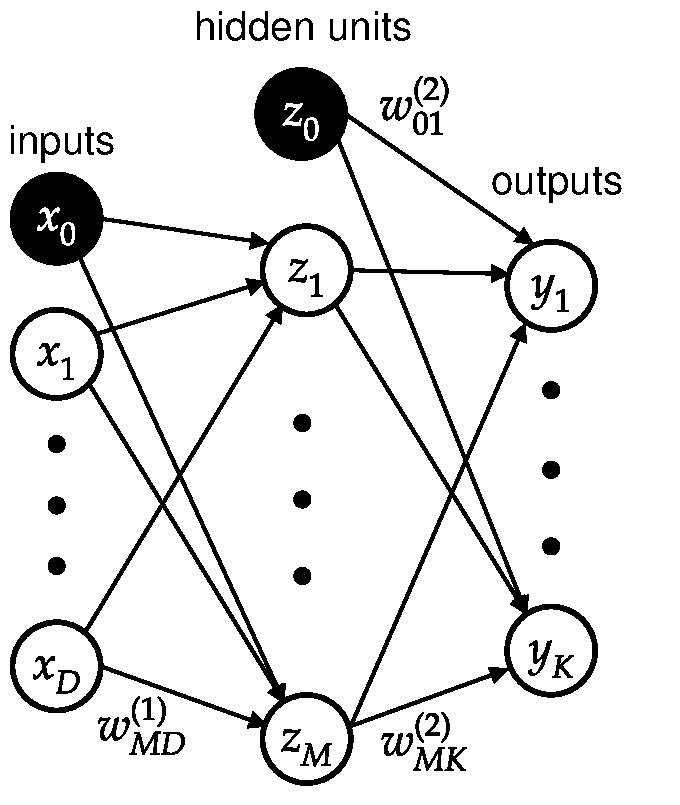
\includegraphics[width=0.4\textwidth]{fully_connected_net.png}
  \caption{Network diagram for a two-layer fully-connected neural network. The input, hidden, and output variables are
  shown as nodes while the weight parameters are the links between them.}%
\label{fig:fully_connected_net}
\end{figure}
%
Often the bias parameters are absorbed into the set of weight parameters by defining an additional input variable
$x_{0}$ whose value is fixed at $x_{0} = 1$ so that Eq~\ref{eq:activations1} becomes
%
\begin{equation}
  a_{j} = \sum_{i=0}^{D} w_{ji}^{(1)} x_{i},
\end{equation}
%
and similarly for the second layer.
%
Written like this then, we can write the overall network function as
%
\begin{equation}
  y_{k}{(\vec{x}, \vec{w})} = \sigma{\left(\sum_{j=0}^{M}w_{kj}^{(2)}
    h{\left(\sum_{i=0}^{D}w_{ji}^{(1)}x_{i}\right)}\right)}
\end{equation}
%
Note that this structure can be easily generalized an arbitrary depth by successively `stacking' these hidden layers.
%
\subsection{Parameter optimization \& Backpropagation}
Given a set of input vectors $\{\vec{x}_{n}\}$ for $n = 1, \ldots, N$, together with a corresponding set of target
vectors $\{\vec{t}_{n}\}$, our goal is to find the values $\vec{w}^{*}$ that minimize some appropriately chosen loss
function $\mathcal{L}(\vec{w})$ that measures the `closeness' between the desired outputs $\vec{t}_{n}$ and the
calculated outputs produced by our network $\vec{y}_n = y(\vec{x}_{n}, \vec{w})$.
%
% In practice, the nonlinearity of the network function $y{(\vec{x_{n}}, \vec{w})}$ causes the loss function
% $\mathcal{L}(\vec{w})$ to be non-convex, leading to local minima to be found.
%
Similar to the gradient descent algorithm discussed in Sec.~\ref{sec:supervised_learning_gradient_descent}, training a
neural network with gradient descent requires the calculation of the gradient of the loss function $\mathcal{L}$ with
respect to the weights $w_{ij}^{k}$ and biases, collectively denoted $\theta$.
%
Then, according to the learning rate $\alpha$, each iteration of gradient descent updates the weights according to
%
\begin{equation}
  \theta^{t+1} = \theta^{t} - \alpha \frac{\partial \mathcal{L}}{\partial \theta}
\end{equation}
%
where $\theta^{t}$ denotes the parameters of the neural network at iteration $t$ of gradient descent.
%
Since the nodes in the hidden layers have no target output, we can't simply define an error function that is specific
to that node. 
%
Instead, any error function for that node will be dependent on the values of the parameters in the previous layers and
following layers.
%
This coupling of parameters between layers often leads to complicated expressions for the gradients and is often slow
in practice.
%
In order to address these issues, an alternative approach is frequently used which relies upon the
\textbf{backpropagation} algorithm, outlined below.
%
For consistency, we adopt the following notations:
%
\begin{itemize}
  \item $X = {\left\{(\vec{x}_{1}, \vec{t}_{1}), \ldots, (\vec{x}_{N}, \vec{t}_{N})\right\}}$: the dataset of $N$
    input-output pairs where $\vec{x}_{i}$ is the input and $\vec{t}_{i}$ is the desired output of the network on input
    $\vec{x}_{i}$
  \item $w_{ij}^{k}$: weight for node $j$ in layer $k$ for incoming node $i$
  \item $w_{0i}^{k} = b_{i}^{k}$: bias for node $i$ in layer $k$ with a fixed output of $z_{0}^{k-1} = 1$ for node $0$ in layer
      $k-1$.
  \item $a_{i}^{k}$ activation (i.e.\ the product sum plus bias) for node $i$ in layer $k$ 
  \item $z_{i}^{k}$: output for node $i$ in layer $k$
  \item $r_{k}$: the number of nodes in hidden layer $k$
  \item $h$: activation function for the hidden layer nodes
  \item $h_{z}$:  activation function for the output layer nodes
\end{itemize}
%
For simplicity, we suppose that the our neural network produces a single, scalar valued output $y$ for a given
vector-valued input $\vec{x}$, and choose a loss function given by the mean-squared error, i.e.\
%
\begin{equation}
  \mathcal{L}(w) = \frac{1}{2N}\sum_{i=1}^{N}{\left(y_{i} - t_{i}\right)}^{2}
\end{equation}
%
Backpropagation then attempts to minimize this loss function with respect to the neural network's weights by
calculating, for each weight $w_{ij}^{k}$, the value of $\frac{\partial \mathcal{L}}{\partial w_{ij}^{k}}$.
%
Since the error function can be decomposed into a sum over individual loss terms for each individual input-output pair,
the derivative can be calculated with respect to each input-output pair individually and then combined at the end (due
to the fact that the derivative of a sum of functions is the sum of the derivatives of each function)
%
\begin{align}
  \frac{\partial \mathcal{L}(X, \theta)}{\partial w_{ij}^{k}}
    &= \frac{1}{N} \sum_{d = 1}^{N} \frac{\partial}{\partial w_{ij}^{k}} {\left(\frac{1}{2}{(y_d - t_d)}^{2}\right)}\\
    &= \frac{1}{N}\sum_{d=1}^{N}\frac{\partial \mathcal{L}_{d}}{\partial w_{ij}^{k}}.
\end{align}
%
Because of this, we can restrict our attention to only one input-output pair and from this the general form for all
input-output pairs can be generated by combining individual gradients.
%
Our loss function then simplifies to 
%
\begin{equation}
  \mathcal{L} = \frac{1}{2}{(y - t)}^{2}
\end{equation}
%
\subsubsection{Derivatives of the Error Function}
We begin by applying the chain rule to the loss function partial derivative
%
\begin{equation}
  \frac{\partial \mathcal{L}}{\partial w_{ij}^{k}} = \frac{\partial \mathcal{L}}{\partial a_{j}^{k}} 
    \frac{\partial a_{j}^{k}}{\partial w_{ij}^{k}}
\end{equation}
%
The first term in the product is often reffered to as the \emph{error} and denoted by $\delta_{j}^{k} \equiv
\partial \mathcal{L}\,/\,\partial a_{j}^{k}$.
%
The second term can be calculated from the fact that
%
\begin{equation}
  a_{j}^{k} = \sum_{j=0}^{r_{k-1}} w_{ij}^{k} z_{j}^{k-1}
\end{equation}
%
to give
%
\begin{align}
  \frac{\partial a_{j}^{k}}{\partial w_{ij}^{k}}
  &= \frac{\partial}{\partial w_{ij}^{k}}{\left(\sum_{l=0}^{r_{k-1}} w_{ij}^{k} z_{l}^{k-1}\right)}\\
  &= z_{i}^{k-1}.
\end{align}
%
Thus, the partial derivative of the loss function $\mathcal{L}$ with respect to a weight $w_{ij}^{k}$ is given by
%
\begin{equation}
  \frac{\partial \mathcal{L}}{\partial w_{ij}^{k}} = \delta_{j}^{k} z_{i}^{k-1},
\end{equation}
%
i.e.\ the partial derivative of a weight is a product of the error term $\delta_{j}^{k}$ at node $j$ in layer $k$, and
the output $z_{i}^{k-1}$ of node $i$ in layer $k-1$.
%
Since the error term $\delta_{j}^{k}$ depends on both the loss function, and as we will show, the values of the error
terms in the next layer, the computation of these terms proceeds backwards from the output layer down to the input
layer which is where the term \emph{backpropagation} (of errors) gets its name.
%
\subsubsection{Output layer}
Starting from the final layer, backpropagation calculates the value\footnote{recall we are considering a one-output
neural network, hence the subscript $1$ and not $j$} $\delta_{1}^{m}$.
%
Expressing the loss function in terms of the value $a_{1}^{m}$ (since $\delta_{1}^{m}$ is a partial derivative with
respect to $a_{1}^{m}$) gives
%
\begin{equation}
  \mathcal{L} = \frac{1}{2} {(t - y)}^{2} = \frac{1}{2} {\left(h_{z}(a_{1}^{m}) - t\right)}^{2}
\end{equation}
%
where again $h_{z}(x)$ is the activation function for the output layer.
%
Applying the partial derivative and using the chain rule gives
%
\begin{equation}
  \delta_{1}^{m} = {\left(h_{z}(a_{1}^{m}) - t\right)} h_{z}^{\prime}(a_{1}^{m}) = (y - t) h_{z}^{\prime}(a_{1}^{m})
\end{equation}
%
and putting it all together, the partial derivative of the loss function $\mathcal{L}$ with respect to a weight in the
final layer $w_{i1}^{m}$ is
%
\begin{equation}
  \frac{\partial E}{\partial w_{i1}^{m}} = \delta_{1}^{m} z_{i}^{m-1} = (y - t) h_{z}^{\prime}(a_{1}^{m}) z_{i}^{m-1}.
  \label{eq:output_layer}
\end{equation}

\subsubsection{Hidden layers}
Now, we calculate the partial derivatives for the hidden layers, again using the multivariate chain rule.
%
Note that for $1 \leq k < m$, the error term $\delta_{j}^{k}$ is:
%
\begin{equation}
  \delta_{j}^{k} = \frac{\partial\mathcal{L}}{\partial a_{j}^{k}} = \sum_{l=1}^{r_{k+1}}
    \frac{\partial\mathcal{L}}{\partial a_{l}^{k+1}}\frac{\partial a_{l}^{k+1}}{\partial a_{j}^{k}},
\end{equation}
%
where $l$ rangers from $1$ to $r_{k+1}$ (the number of nodes in the next layer).
%
Plugging in the error term $\delta_{l}^{k+1}$ gives
%
\begin{equation}
  \delta_{j}^{k} = \sum_{l=1}^{r_{k+1}} \delta_{l}^{k+1} \frac{\partial a_{l}^{k+1}}{\partial a_{j}^{k}}.
\end{equation}
%
% and by the definition of $a_{l}^{k+1}$,
Recalling that
%
\begin{equation}
  a_{l}^{k+1} = \sum_{j=1}^{r_{k}} w_{jl}^{k+1} h(a_{j}^{k})
\end{equation}
%
where $h(x)$ is the activation function in the hidden layers, we are left with
%
\begin{equation}
  \frac{\partial a_{l}^{k+1}}{\partial a_{j}^{k}} = w_{jl}^{k+1} h^{\prime}(a_{j}^{k}).
\end{equation}
%
Plugging this into the above equation gives a final equation for the error term $\delta_{j}^{k}$ in the hidden layers,
a result known as the \emph{backpropagation formula}:
%
\begin{equation}
  \delta_{j}^{k} = \sum_{l=1}^{r_{k+1}} \delta_{l}^{k+1} w_{jl}^{k+1} h^{\prime}(a_{j}^{k}) 
    = h^{\prime}(a_{j}^{k})\sum_{l=1}^{r_{k+1}} w_{jl}^{k+1} \delta_{l}^{k+1}
    \label{eq:hidden_layers}
\end{equation}
%
Putting this all together we get the partial derivative of the loss function $\mathcal{L}$ with respect to a weight in
the hidden layers $w_{ij}^{k}$ for $1 \leq k < m$:
%
\begin{equation}
  \frac{\partial \mathcal{L}}{\partial w_{ij}^{k}} = \delta_{j}^{k} z_{i}^{k-1} = h^{\prime}(a_{j}^{k})z_{i}^{k-1}
    \sum_{l=1}^{r_{k+1}} w_{jl}^{k+1}\delta_{l}^{k+1}.
    \label{eq:loss_terms}
\end{equation}
%
For completeness, we include the complete algorithm in Alg.~\ref{alg:backprop_algorithm}.
%
\begin{algorithm}[htpb]
    \SetKwProg{Fn}{def}{\string:}{}%
    \SetKwFunction{Range}{range}%
    \SetKwFor{For}{for}{\string:}{}%
    \SetKwIF{If}{ElseIf}{Else}{if}{:}{elif}{else:}{}%
    \SetKwFor{While}{while}{:}{fintq}%
    \AlgoDontDisplayBlockMarkers\SetAlgoNoEnd\SetAlgoNoLine%
    \DontPrintSemicolon%
    \SetKwInOut{Input}{input}\SetKwInOut{Output}{output}%
    \caption{Backpropagation Algorithm}%
    \Input{A data set $X = \{(\vec{x}_{1}, t_{1}), \ldots, (\vec{x}_{N}, t_{N})\}$ consisting of $N$ input-output
    pairs, the learning rate $\alpha$, the loss function $\mathcal{L}$, and the activation function $h$}\;
    %
    \begin{enumerate}
      \item \textbf{Forward pass:} For each input-output pair $(\vec{x}_{d}, t_{d})$, store the results $y_{d}$,
        $a_{j}^{k}$, and $z_{j}^{k}$ for each node $j$ in layer $k$ by proceeding from the input layer to the output
        layer $m$.\;
      \item \textbf{Backward pass:} For each input-output pair $(\vec{x}_{d}, t_{d})$, store the results $\partial
        \mathcal{L}_{d}\,/\, \partial w_{ij}^{k}$ for each weight $w_{ij}^{k}$ connecting node $i$ in layer $k - 1$ to
        node $j$ in layer $k$ by proceeding from layer $m$, the output layer, to the input layer.\;
        \begin{itemize}
          \item Evaluate the error term for the final layer $\delta_{1}^{m}$ by using Eq.~\ref{eq:output_layer}.\;
          \item Backpropagate the error terms for the hidden layers $\delta_{j}^{k}$, working backwards from the final
            hidden layer $k = m - 1$ by repeatedly using Eq.~\ref{eq:hidden_layers}.\;
          \item Evaluate the partial derivatives of the individual error $\mathcal{L}_{d}$ with respect to $w_{ij}^{k}$
            by using Eq.~\ref{eq:loss_terms}.\;
        \end{itemize}
      \item \textbf{Combine individual gradients:} for each input-output pair $\frac{\partial \mathcal{L}_{n}}{\partial
        w_{ij}^{k}}$ to get the total gradient $\frac{\partial \mathcal{L}(X, \theta)}{\partial w_{ij}^{k}}$ for the
          entire set of input-output pairs using\;
          \begin{equation*}
            \frac{\partial \mathcal{L}(X, \theta)}{\partial w_{ij}^{k}} =
              \frac{1}{N}\sum_{d=1}^{N}\frac{\partial}{\partial w_{ij}^{k}} {\left(\frac{1}{2}{(y_n -
                t_{n})}^{2}\right)} = \frac{1}{N}\sum_{d=1}^{N}\frac{\partial \mathcal{L}_{d}}{\partial w_{ij}^{k}}
          \end{equation*}
    \end{enumerate}%
\label{alg:backprop_algorithm}
\end{algorithm}

\section{Convolutional Neural Networks}
Convolutional neural networks (CNNs or ConvNets) is a generic term used to describe any neural network whose
architecture includes convolutional layers. 
%
Consequently, ConvNets are similar in many ways to the fully-connected feed-forward layers previously discussed, and
are almost always used in conjunction with some combination of fully-connected layers.
%
An example architecture can be found in Fig.~\ref{fig:conv_net}.
%
The difference now is that we expect our input data to have some rectangular structure (e.g.\ two-dimensional images),
which are often represented as a three-dimensional volume of shape
$\mathrm{height}\times\mathrm{width}\times\mathrm{depth}$ where $\mathrm{height}$ and $\mathrm{width}$ are, as
we would expect, the height and width of the input image, and $\mathrm{depth}$ usually refers to the number of
\emph{color channels} (i.e.\ RGB) of the image.
%
For example, if we are dealing with a typical two-dimensional RGB image, then $\mathrm{depth} = 3$, which we could
represent as a three-dimensional volume of $\mathrm{height}\times\mathrm{width}\times[\mathrm{red},
\,\mathrm{green},\, \mathrm{blue}]$ pixels.

Additionally, in contrast to fully-connected networks, ConvNets combine three architectural ideas to ensure some degree
of shift and distortion invariance~\cite{lecun1995convolutional}:
%
\begin{itemize}
  \item \emph{Local receptive fields}
  \item \emph{Shared weights} (or weight replication)
  \item Spatial or temporal subsampling (or \emph{pooling})
\end{itemize}
%A
% The difference now is that we expect our input data to have some rectangular structure (e.g.\ two-dimensional images),
% which are often represented as a three-dimensional volume of shape
% $\mathrm{height}\,\times\,\mathrm{width}\,\times\,\mathrm{depth}$ where $\mathrm{height}$ and $\mathrm{width}$ are, as
% we would expect, the height and width of the input image, and $\mathrm{depth}$ usually refers to the number of
% \emph{color channels} (i.e.\ RGB) of the image.
% %
% For example, if we are dealing with a typical two-dimensional RGB image, then $\mathrm{depth} = 3$, which we could
% represent as a three-dimensional volume of $\mathrm{height}\,\times\,\mathrm{width}\,\times\,[\mathrm{red},
% \,\mathrm{green},\, \mathrm{blue}]$ pixels.
%
\subsection{Local receptive fields}
When dealing with high-dimensional inputs such as images, it is impractical to fully-connect each neuron to all neurons
in the previous volume because such a network architecture does not take into account the spatial structure of the
data.
%
Convolutional networks exploit spatially local correlation by enforcing a sparse local connectivity pattern between
neurons of adjacent layers: each neuron is connected to only a small region of the input volume.
%
The spatial extent of this connectivity is a hyperparamter, known as the \emph{local receptive field}.
%
The connections are local in space (along the height and width), but always extend along the entire depth of the input
volume.

We begin with an example.
%
Suppose we take as input a $16\times16$ square of pixels, corresponding to an image.
%
Proceeding as before, we connect the input pixels to a layer of hidden units, with the exception that now we only make
connections in small, localized regions of the input image.
%
Explicitly, each neuron in the first hidden layer will be connected to a small region of the input units, say, for
example, a $4\times4$ region, corresponding to $16$ input pixels.
%
The region in the input image is known as the \emph{local receptive field} for the hidden unit.
%
This local receptive field can be understood as a little window on the input pixels, with each connection learning a
weight.
%
% Each individual hidden unit then learns to analyze its particular local receptive field.
%
% The local receptive field is then slid (or \emph{convolved}) across the entire input image, with each local receptive
% field corresponding to a different hidden unit in the first hidden layer.
% %
% This process can be seen in Fig.~\ref{fig:local_receptive_field}, and is repeated for each individual node in the first
% hidden layer.
%
During the forward pass through our network, each filter is convolved across the height and width of the input volume
(as illustrated in Fig.~\ref{fig:local_receptive_field}) computing the dot product between the entries of the filter
and the input, producing a two-dimensional activation map of that filter.
%
As a result, the network learns filters that activate when it detects some specific type of feature at some spatial
position in the input.
%
Stacking these activation maps for all filters along the depth dimension forms the full output volume of the
convolution layer.
%
All together, there are three hyperparameters that control the size of the output volume of the convolutional layer:
the \emph{depth}, \emph{stride length}, and \emph{zero-padding}.
%
The \emph{depth} of the output volume controls the number of neurons in a layer that connect to the same local
receptive field of the input volume.
%
These neurons learn to activate for different features in the input, e.g.\ various oriented edges or blobs of color.
%
The \emph{stride length}, $S$ (chosen as $S = 1$ in Fig.~\ref{fig:local_receptive_field}), controls how depth columns
around the spatial dimensions (height and width) are allocated.
%
This can be understood as the distance by which the local receptive field is moved to construct a new hidden unit.
%
Note that in our example we chose $S=1$, but it is not uncommon to use different values (typically $S = 1, 2$),
depending on the particulars of the problem at hand.
%
Finally, it is sometimes convenient to pad the input with zeros on the border of the input volume.
%
This hyperparamter is known as the \emph{zero-padding}, and denoted by $P$.
%
The spatial size of the output volume can be computed as a function of the input volume size $W$, the spatial size of
the local receptive field (also known as the \emph{kernel} or \emph{filter} size), $K$, the stride length with which
they are applied $S$, and the amount of zero-padding $P$ used on the border.
%
The equation for calculating how many neurons `fit' inside a given volume is then given by
%
\begin{equation}
  \frac{W - K + 2P}{S} + 1
\end{equation}
%
If this number is not an integer, then the strides are incorrect and the neurons cannot be tiled to fit across the
input volume in a symmetric manner.
%
In general, setting the zero padding to be $P = (K - 1) / 2$ when the stride is $S=1$ ensures that the input volume and
output volume will have the same size spatially.
%
\begin{figure}[htpb]
  \centering
  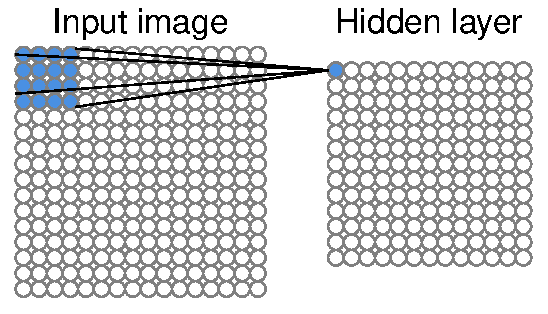
\includegraphics[width=0.48\textwidth]{conv_net/local_receptive_fields1.pdf}
  \hfill
  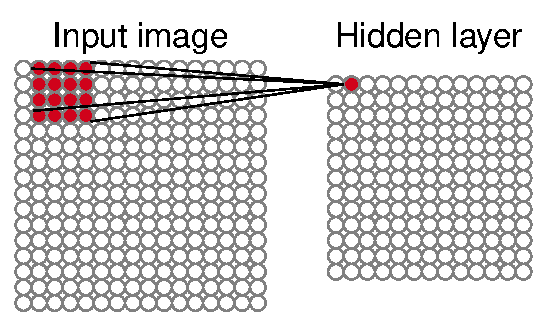
\includegraphics[width=0.48\textwidth]{conv_net/local_receptive_fields2.pdf}
  \caption{Illustration of the local receptive fields in the input image and their corresponding weights in the first
    hidden layer. Additionally, we can see how these local receptive fields are slid across the input image to
  construct additional units in the hidden layer.}%
  \label{fig:local_receptive_field}
\end{figure}
%
\subsection{Shared weights}
A parameter sharing scheme is used in convolutional layers to control the number of free paramters.
%
This scheme relies on the reasonable assumption that if a patch feature is useful to compute at some spatial position,
then it should also be useful to compute at other positions.
%
Equivalently, if we denote a single two-dimensional slice of depth as a \emph{depth slice}, we constrain the neurons in
each depth slice to use the same weights and biases.
%
Since all neurons in a single depth slice share the same parameters, the forward pass in each depth slice of the
convolutional layer can be computed as a convolution of the neuron's weights with the input volume.
%
Because of this, the sets of weights which are convolved with the input are often referred to as a \emph{filter} or
\emph{kernel}.
%
The result of this convolution is then called the \emph{activation map}, and the set of activation maps for each
different filter are stacked together along the depth dimension to produce the output volume.
%
This idea of parameter sharing helps contribute to the translation invariance of the CNN architecture.
%
\subsection{Pooling Layers}
Another important concept of CNNs is pooling, which is a form of non-linear down-sampling.
%
This concept is implemented in what we call \emph{pooling layers}, which are usually used immediately following
convolutional layers.
%
The pooling layer serves to progressively reduce the spatial size of the representation, to reduce the number of
parameters, memory footprint and amount of computation in the network, and hence to also control
overfitting~\cite{scherer2010evaluation,2014arXiv1412.6806S}.
%
In doing so, the pooling operation provides another form of translation invariance.
%
What these layers do is simplify the information in the output from the convolutional layer by summarizing some region
of neurons in the previous layer.
%
The most common form is a pooling layer with filters of size $2\times2$ applied with a stride of $2$ downsamples at
every depth slice in the input by $2$ along both the height and width, discarding $75\%$ of the activations.
%
One common type of pooling layer is known as \emph{max pooling}, in which a pooling unit simply outputs the maximum
activation in the $2\times2$ input region.
%
This behavior can be seen in Fig.~\ref{fig:max_pool}.
%
\begin{figure}[htpb]
  \centering
  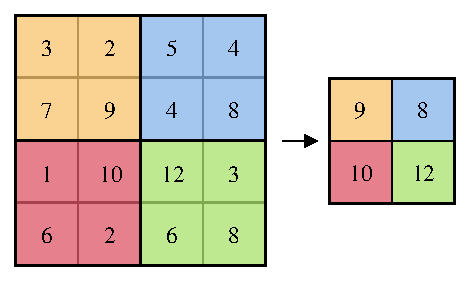
\includegraphics[width=0.6\textwidth]{max_pooling}
  \caption{Illustration of a $2\times2$ max pooling layer.}%
\label{fig:max_pool}
\end{figure}
%
\subsection{Hyperparameters}%
\label{subsec:ml_cnn_hyperparameters}
Since CNNs use more hyperparameters than typical feed-forward fully-connected neural networks, it is often difficult to
determine what values are appropriate for the problem at hand.
%
One idea to keep in mind is that since the size of the feature maps decreases with increasing network depth, layers
closer to the input layer will tend to have fewer filters while deeper layers will usually have more.
%
The number of feature maps directly controls the layers' capacity and depends on the number of available examples and
the complexity of the problem being studied.
%
It is common to use small filters (e.g. $3\times3$ or at most $5\times5$) using a stride of $S=1$, and padding
the input volume with zeros in such a way that the convolutional layer does not alter the spatial dimensions of the
input.
%
Since the pooling layers are in charge of downsampling the spatial dimensions of the input, a common setting is to use
max-pooling with $2\times2$ receptive fields (i.e. $K = 2$), and with a stride of $S = 2$.
%
With this choice of hyperparameters, exactly $75\%$ of the activations in an input volume are discarded (since we
downsample by $2$ in both height and width).
%
% Note that in Fig.~\ref{fig:local_receptive_field}, we have implicitly chosen a \emph{stride length} of $S = 1$, i.e.\
% the local receptive field is being moved by one pixel at a time.
% %
% % The stride lengh controls how depth columns around the spatial dimensions (height and width) are allocated.
% %
% This value is merely a choice and it is not uncommon to use different values of the stride length (typically $S = 1,
% 2$) depending on the particulars of the problem at hand.
%
%
% Note that larger stride lengths correspond to smaller output volumes spatially.

% The difference now is that we expect our input data to have some rectangular structure (e.g.\ two-dimensional images),
% which are often represented as a three-dimensional volume of shape
% $\mathrm{height}\,\times\,\mathrm{width}\,\times\,\mathrm{depth}$ where $\mathrm{height}$ and $\mathrm{width}$ are, as
% we would expect, the height and width of the input image, and $\mathrm{depth}$ usually refers to the number of
% \emph{color channels} (i.e.\ RGB) of the image.
% %
% For example, if we are dealing with a typical two-dimensional RGB image, then $\mathrm{depth} = 3$, which we could
% represent as a three-dimensional volume of $\mathrm{height}\,\times\,\mathrm{width}\,\times\,[\mathrm{red},
% \,\mathrm{green},\, \mathrm{blue}]$ pixels.
%
% Explicitly, a convolutional layer's parameters consist of a set of learnable filters.
% %
% Every filter is small spatially (along the height and width dimensions), but extends through the full depth of the
% input volume, e.g.\ for an input image of shape $32\,\times\,32\,\times\,3$, a filter in the first convolutional layer
% may have shape $5\,\times\,5\,\times\,3$.
% %
% During the forward-pass through our network, we slide (or \emph{convolve}), each filter across the height and width of
% the input volume and compute dot products between the entries of the filter and the input at any position.
% %
% As we slide the filter over the height and width of the input volume we produce a two-dimensional activation map that
% gives the responses of that filter at every spatial position


%
% They are composed of hidden units with learnable weights and biases.
%
% Each unit receives an input, performs a dot product and optionally follows it with some non-linear function.
%
% Convolutional neural networks combine three architectural ideas to ensure some degree of shift and distortion
% invariance~\cite{lecun1995convolutional}:
% %
% \begin{itemize}
%   \item Local receptive fields
%   \item Shared weights (or weight replication)
%   \item Spatial or temporal subsampling
% \end{itemize}
%

% Each unit of a convolutional layer receives inputs from a set of units located in a small neighborhood in the previous
% layer.
% %
% The spatial extent of this connectivity is a hyperparameter called the \textbf{receptive field} (equivalently, the
% \emph{filter} or \emph{kernel} size) of the unit.
%
% The difference now is that we expect as input to our network some vector that has a rectangular structure, such as a
% two-dimensional image of pixels.
%
% These features in particular make
\section{Conclusion}
In this chapter we have introduced the concept of machine learning and provided a broad overview of some of the topics
that will be used in the following chapters.
%
The information provided here is by no means exhaustive, and for further reference I highly suggest the excellent book
by Bishop~\cite{Bishop:2006:PRM:1162264}.
%
Moreover, for those interested, there is no shortage of online materials available and a quick google search
will provide an endless collection of useful resources.
%
In many ways, we have just barely scratched the surface of machine learning and it would be nearly impossible to
include everything in this work.
%
The idea of applying ideas from machine learning to problems in physics has only just recently begun to be explored and
it is quickly becoming a very active area of research.
%


\end{document}
